\pagenumbering{arabic}
\chapter{Einleitung}
In den vergangenen Jahren war ein massiver Zunahme des generierten Datenaufkommens zu beobachten \cite{EMC2014}. Viele Projekte, Unternehmen und Institutionen haben Zugriff auf eine gewaltige Menge an Daten. Diese wächst immer schneller an. 2004 analysierte Google circa 100 Terabyte pro Tag \cite{Dean2004}. Bis zum Jahr 2008 war die täglich zu analysierende Datenmenge bereits auf 20 Petabyte angewachsen \cite{Dean2008}. Das Sloan Digital Sky Survey, das ein Viertel des Himmels astronomisch erkundet, hat seit 1998 insgesamt 116 Terabyte an astronomischen Daten gesammelt \cite{York2000, Alam2015}. Jede Nacht kommen circa 250 Gigabyte neu hinzu \textcolor{blue}{Quelle: Herr Prof. Freytags VL, dort angegebene Quelle ist offline. Wie angeben?}. Ein weiteres Beispiel ist das 1000 Genomes Project \cite{Baker2010}, das zwischen 2008 und 2013 insgesamt 464 Terabyte Daten zum menschlichen Genom sammelte. Insgesamt werden die Datenmengen weiter stark zunehmen, für das Jahr 2020 wird eine weltweites Datenaufkommen von 44 Zettabyte prognostiziert \cite{EMC2014}. 
Diese Entwicklung offenbart diverse neue Herausforderungen bei der Speicherung, Verarbeitung und Analyse von Daten. Dabei spielt die möglichst schnelle Verarbeitung von stetig generierten Daten eine große Rolle. Diese muss im Gegensatz zur Verarbeitung bereits gespeicherter Daten abhängig vom aktuellen Datenaufkommen skalieren. Aktuelle Datenverarbeitungssysteme wie Apache Hadoop \cite{HadoopWebsite} und Apache Flink \cite{FlinkWebsite} bieten diese Möglichkeit der Datenflussanalyse und ermöglichen eine flexible Analyse der Daten. Kern dieser Systeme ist eine Implementierung des Map-Reduce Paradigmas \cite{Dean2008} sowie die Nutzung von \textit{User Defined Functions}. Diese ermöglichen eine parallele Abarbeitung von Arbeitsschritten in einem direkten, azyklischen Graphen. Der DAG wird zuvor aus dem vom User bereitgestellten Quellcode erzeugt. Die durch diese Architektur erreichbare, massiv parallelisierbare Ausführung der Datenanalyse ermöglicht die Nutzung von Clustern. Somit wird eine skalierbare Infrastruktur genutzt, die wiederum eine skalierte Nutzung der Datenverarbeitungssysteme ermöglicht. Diese Systeme können auch die weiterhin wichtige Nutzung und Analyse von bereits konsistent gespeicherten Daten unter Nutzung des parallelen Verarbeitungsansatzes durchführen. Dies ist insbesondere deshalb notwendig, da traditionelle Datenbanksysteme große Datenmengen nicht immer in akzeptabler Form und Verarbeitungszeit verarbeiten können \cite{Jacobs2009}.
\newline
Das Hauptproblem bei der Verarbeitung von großen Datenmengen auf einzelnen Maschinen entsteht, wenn die zu verarbeitende Datenmenge die Hauptspeichergröße übersteigt. In diesem Fall müssen die nicht in den Hauptspeicher speicherbaren Daten zur Verarbeitungszeit nachgeladen werden, was die Verarbeitungszeit aufgrund der unterschiedlichen Beschaffenheit der verschiedenen Speicherebenen extrem verlängert. Um diese "Speicherklippe" zu umgehen, werden zunehmend parallelisierbare Ansätze der Datenverarbeitung verfolgt.
Im Rahmen dieser Bachelorarbeit sollen demzufolge ein traditioneller und ein massiv parallelisierbarer Ansatz bei der Verarbeitung von großen Datenmengen untersucht werden. So soll eine Abschätzung der Leistungsfähigkeit, Vorteile und Nachteile beider Ansätze ermittelt werden. Der Vergleich beider Ansätze wird am Beispiel eines Algorithmus zur Approximierung von Pixelzeitreihen durchgeführt. Dieser wird im Rahmen des Projekts GeoMultiSens\cite{GeoMultiSensWebsite} zur Analyse der Veränderung der Flora in einer geographischen Region genutzt. Dabei werden durch Landsat-Satelliten Satellitenaufnahmen bereitgestellt, die nach der Aufbereitung durch vorgestellte Algorithmen ausschnittweise untersucht werden. Nach der Analyse werden anschließend mithilfe des Algorithmus auf Basis der approximierten Werte Prognosen zur weiteren Entwicklung der Flora der untersuchten Region gestellt. Dabei werden bei einer Analyse mehrere Szenenausschnitte derselben geographischen Region analysiert. Dabei müssen große Datenmengen verarbeitet werden, so dass sich die Nutzung eines aktuellen Datenverarbeitungssystems anbietet. Bei dieser Bachelorarbeit wird als Vertreter der massiv parallelisierbaren Datenverarbeitungssysteme Apache Flink genutzt.
\newline
Es werden drei unterschiedliche Implementierungen des Algorithmus untersucht, die sich hinsichtlich der eingesetzten Technologien und Programmiersprachen unterscheiden. Die zugrunde liegende Methodik, die der Algorithmus implementiert, ist bei allen untersuchten Varianten identisch. Als Basis wird die bereits implementierte und in der Praxis genutzte Python-Implementation genutzt. Sie sollte somit die untere Schranke der Leistungsmessungen darstellen. Die zweite und dritte Variante werden in Flink implementiert. Diese beiden Varianten unterscheiden sich bezüglich der genutzten Programmiersprache. \textcolor{blue}{Zur Implementierung der zweiten Variante wird Java-Schnittstelle von Flink genutzt, zur Umsetzung von Variante drei die Python-Schnittstelle.} Schließlich werden alle drei Varianten unter identischen Bedingungen getestet. Dies bedeutet, dass sowohl die Testumgebung als auch die Testdaten identisch sein sollen. Dabei sollen alle Varianten sowohl auf einer leistungsfähigen Einzelmaschine als auch mit einem Cluster von Maschinen getestet werden. Ausgehend von den Untersuchungen und den ermittelten Ergebnissen soll nachfolgend eine Bewertung der drei Implementierungsvarianten des Algorithmus vorgenommen werden. Dabei sollen insbesondere die Größe der Ausgangsdatenmenge, die genutzte Hardware sowie die Größe der untersuchten Bildausschnitte in Bezug zu den Ergebnissen gesetzt werden.

%----------------------------------------------------------------------------------

\chapter{Grundlagen}

Die Basis für die Satellitenbildanalyse mittels Apache Flink bilden zum einen Konzepte aus der Geographie, zum anderen Strukturen und Vorgehensweisen aus der Informatik. Während die geographische Komponente insbesondere bei der Aufnahme der Satellitenbilder sowie bei der inhaltlichen Konzeption der Analysen sowie der Bereinigung der Daten vertreten ist, ist die Informatik für eine technisch korrekte und effiziente Umsetzung der geographischen Konzepte verantwortlich. Nachfolgend werden zuerst die geographischen Grundlagen der Fernerkundung erläutert. Dies umfasst insbesondere die technische Spezifikation der Aufnahmegeräte der eingesetzten Satelliten sowie wichtige Verfahren zur Datenaufbereitung sowie zur Datenanalyse. Anschließend wird ein Überblick über parallele Datenverarbeitungssysteme gegeben. Dieser umfasst auch die Eigenschaften von Big Data sowie eine konzeptuelle Beschreibung der Datenanalyseplattform Apache Flink. Abschließend wird Apache Flink aus der Entwicklerperspektive betrachtet. Dabei werden insbesondere Eigenschaften der Plattform beschrieben, die bei der Entwicklung von Programmen auf Basis von Flink von Bedeutung sind. Des weiteren wird die Programmiersprache Python betrachtet.

\section{Grundlagen der Satellitenbildanalyse}
\subsection{Fernerkundung mithilfe des Landsat-Satellitensystems}

Als Fernerkundung wird \textcquote{DIN18716}{die Gesamtheit der Verfahren zur Gewinnung von Informationen über die Erdoberfläche oder anderer nicht direkt zugänglicher Objekte durch Messung und Interpretation der von ihr ausgehenden (Energie-) Felder} verstanden. Fernerkundungssatelliten verfügen über verschiedene Aufnahmesysteme, die durch multispektrale Messungen von emittierter elektromagnetischer Strahlung eine berührungsfreie Beobachtung der Erdoberfläche ermöglichen. Bei der multispektralen Messung werden von Sensoren registrierte spektrale Signaturen einzelnen Bereichen des elektromagnetischen Spektrums zugeordnet. Das Resultat sind mehrere spektrumsspezifische, simultan aufgenommene Satellitenbilder, die nur das aufgefangene Licht eines spezifischen Spektralbereichs, auch Spektralband genannt, zeigen. Die Art und Qualität der Aufnahmesensoren ist dabei abhängig vom Typ des Satelliten. 

Die Ausgangsdaten für die Untersuchungen in dieser Bachelorarbeit wurden von Satelliten des Landsat-Satellitensystems aufgenommen. Der erste Landsat-Satellit Landsat 1 wurde 1972 gestartet. Seitdem wurden die Sensoren und die Satelliten kontinuierlich weiterentwickelt. Aktuell sind Landsat 7 und, im Rahmen der Landsat Data Continuity Mission, Landsat 8 im Einsatz. Landsat 8 nutzt in der aktuellen Generation zwei verschiedene Instrumente zur Fernerkundung. Den Operational Land Imager (OLI) und die Thermal Infrared Sensors (TIRS). 

Der OLI erfasst emittierte elektromagnetische Strahlung im Spektralbereich von 0,433 µm bis 1,390 µm unterteilt in acht Spektralkanäle sowie einen panchromatischen Kanal. Es werden mehr als 7000 Detektoren pro Spektralband genutzt, um eine bessere Bildqualität zu bieten als frühere Systeme \cite{Markham2004}. Neben den klassischen Farbspektren Blau, Grün und Rot nutzt Landsat-8 ein weiteres Band, das speziell für die Fernerkundung von Küsten genutzt wird. Außerdem verfügt Landsat-8 über drei Infrarotbänder, die nahes und mittleres Infrarotlicht registrieren, sowie ein weiteres Infrarotband, das auf die Beobachtung von Cirruswolken spezialisiert ist. Der panchromatische Kanal registriert elektromagnetische Strahlung mit Wellenlängen von 0,500 µm bis 0,680 µm. Dieser Spektralbereich entspricht etwa dem des menschlichen Auges. Aufgrund des, im Vergleich zu den einzelnen Farbfrequenzbändern, breiten abgedeckten Spektralbereichs ist eine höhere Auflösung der Bilder möglich.

Die Thermal Infrared Sensors (TIRS) \cite{Chaudhary2011} umfassen zwei Thermalkanäle. Diese erfassen im Gegensatz zu den Multispektralkanälen elektromagnetische Emissionen mit Wellenlängen zwischen 10,30 µm und 12,50 µm, also langwellige Infrarotstrahlung. Dies ist insbesondere für die Beobachtung von Wolken nützlich. Die Kantenlänge der einzelnen Pixel beträgt 100 Meter. Diese kann nachträglich auf 30 Meter angeglichen werden, um eine bessere Kompatibilität mit den Aufnahmen der Multispektralbänder zu gewährleisten.

Landsat 8 sendet pro Tag 400 Aufnahmen der Erdoberfläche, auch Szenen genannt, an die Bodenstation. Eine Aufnahme zeigt dabei eine geographische Region der Erde mit einer Ost-West-Ausdehnung von 185 Kilometer. Dies entspricht 100 nautischen Meilen. Die Nord-Süd-Ausdehnung einer Szene beträgt circa 174 Kilometer 

Durchschnittlich wird jede Region der Erde alle \textcolor{blue}{16 (?)} Tage überflogen \cite{Irons2012}.

Die von Landsat-Satelliten aufgezeichneten und übermittelten Bilder müssen jedoch vor der Durchführung von Analysen aufbereitet werden.

%----------------------------------------------------------------------------------

\subsection{Aufbereitung und Analyse von Satellitenbildern}
%Szenen müssen aufbereitet werden
Die durch die Landsat-Satelliten aufgezeichneten und an die Bodenstationen übermittelten Szenen müssen vor ihrer Nutzung aufbereitet werden. Dadurch wird im Allgemeinen die Bildqualität verbessert, da externe Störfaktoren und eventuelle interne Fehlfunktionen ausgeglichen werden können. Es wird zwischen radiometrischen und die geometrischen Aufbereitungen unterschieden. Bei der radiometrischen Aufarbeitung werden digitale Werte wie zum Beispiel die Helligkeit der Szene angepasst. 

%Wie werden sie aufbereitet? Warum werden sie aufbereitet?
Im Rahmen der geometrischen Aufbereitung sollen die Folgen einer eventuellen Fehlpositionierung des Satelliten korrigiert werden. Um die Szenen sinnvoll analysieren zu können, müssen sie korrekt und genau positioniert sein. Dies gilt insbesondere bei der Analyse einer Serie von Szenen derselben geographischen Region. Um eine normierte Positionierung der Szenen zu schaffen, werden aus jeder Szene, die einen Teil der zu analysierenden geographischen Region beinhaltet, quadratische Teile der Originalszene ausgeschnitten. Diese ausgeschnittenen Bereiche der ursprünglichen Szene werden Kacheln genannt. Dann wird jeder Pixel der Kachel auf die Zugehörigkeit zum Zielgebiet geprüft. Wenn ein Pixel relevant ist, wird er anhand seiner, aus der Position des Satelliten zum Aufnahmezeitpunkt ermittelten, Position in einem finalen Bild hinzugefügt. Dies garantiert eine einheitliche Grundlage für die Analyse der Zielregion.

Zusätzlich zu Fehlpositionierungen des Satelliten und den sich daraus ergebenden Abweichungen müssen möglicherweise noch weitere Störfaktoren durch die Aufbereitung gemindert werden. Hierzu zählen zum Beispiel durch die Atmosphäre verursachte Verschlechterungen, die aus Interferenzen innerhalb der Atmosphäre zwischen Erdoberfläche und dem Satelliten resultieren. Diese sollen korrigiert werden, um ein genaueres Satellitenbild zu erhalten. Techniken um diese Verbesserung zu erreichen sind beispielsweise das Strahlungstransfermodell, die bildbasierte atmosphärische Korrektur und die Histogramm-Minimum-Methode. Es ist individuell von der Szene und den zur Verfügung stehenden Metadaten abhängig, mit welcher Methode die nützlichste Verbesserung erreicht werden kann.

%Bedeutung für mich/ Ausblick auf steigende Datenmengen
Die Aufbereitung von Satellitenbildern muss vor einer wissenschaftlichen Analyse erfolgen, damit die Szenen unabhängig von Witterungseinflüssen, Atmosphäreninterferenzen, Fehlpositionierungen und sonstiger Störfaktoren untersucht werden können. Durch die zunehmend bessere Qualität von Satellitenbildern, die durch Fernerkundungsatelliten aufgezeichnet werden \cite{Markham2004}, können detailliertere Analysen getätigt werden. Jedoch steigt mit zunehmender Größe der Bilddateien auch der Rechenaufwand, um die Szenen aufzubereiten und zu analysieren. Mit zunehmender Datenmenge wird eine massiv parallelisierbare Vorgehensweise bei der Aufbereitung und der Analyse von Satellitenbildern attraktiver. Denn verteilte Systeme lassen sich meist kostengünstiger und flexibler erweitern als einzelne Maschinen, so dass das System bei einer unerwartet großen Datenmenge schnell erweitert werden kann. Dadurch lässt sich eine schnellere Ausführung der Prozesse erreichen.

%----------------------------------------------------------------------------------

\section{Parallele Datenverarbeitungssysteme}
%Einleitung
Seit mehreren Jahren ist ein massiver Anstieg der global produzierten Datenmengen zu beobachten \cite{EMC2014}. Diese Menge an Daten ist mithilfe traditioneller Methoden der sequentiellen, stapelweisen Datenverarbeitung nicht effizient zu verarbeiten. Aus diesem Grund wird eine verteilte Verarbeitung von Daten in vielen Bereichen zunehmend populär. Dies gilt insbesondere für Daten, die gemäß der in Sektion~\ref{sec:BigData} beschriebenen Kriterien als Big Data klassifiziert werden. Um eine parallele Verarbeitung von Big Data zu ermöglichen, wurden bestehende parallele Datenverarbeitungsmechanismen erweitert. Insbesondere das Map-Reduce Paradigma \cite{Dean2004} bewirkte eine grundlegende Veränderung bei der Vorgehensweise zur Verarbeitung großer Datenmengen. In der Folge wurde Map-Reduce erweitert und flexibler einsetzbar. Diese Entwicklung wird in Sektion~\ref{sec:GrosseDatenmengen} erläutert. Eines der Systeme auf Basis von Map-Reduce ist Apache Flink \cite{FlinkWebsite}. Es ermöglicht eine massiv parallelisierbare und echtzeitnahe Verarbeitung von großen Datenmengen. Die konzeptionelle Struktur von Apache Flink wird in der Sektion~\ref{sec:ApacheFlink} beschrieben. Als Alternative zu parallelen Ansätzen existiert die bisherigen sequentiellen bzw. händisch parallelisierbaren Ansatz. Dieser wird am Beispiel der Programmiersprache Python in Sektion~\ref{sec:Python} kurz beschrieben.

\subsection{Bedeutung und Eigenschaften von Big Data}
\label{sec:BigData}
%Einleitung - Eigenschaften von Big Data
Für das Jahr 2020 wird in der Folge der weltweit zunehmenden Generierung von Daten ein weltweites Datenaufkommen von 44 Zettabyte prognostiziert \cite{EMC2014}. Zusätzlich zu dieser schnell wachsenden Menge an verfügbaren Daten wächst auch der Bedarf diese nutzbringend zu analysieren. Insbesondere Forschungseinrichtungen und Unternehmen verfügen über immer größere Datenmengen und versuchen Erkenntnisse aus diesen zu gewinnen. Ein weiterer Teil dieser Daten wird durch die zunehmende Verbreitung des Internets der Dinge und die zunehmende Nutzung von Internetdiensten durch Konsumenten generiert. Traditionelle Methoden der Datenanalyse reichen jedoch nicht mehr aus, um diese Daten auszuwerten. 

Dies resultiert aus den vier Eigenschaften, durch die Big Data definiert werden. Insbesondere die drei Charakteristika Volumen (engl. \textit{volume}), Komplexität (engl. \textit{variety}) sowie die echtzeitnahe Verfügbarkeit und schnelle Verarbeitung (engl. \textit{velocity}) von Daten, die bereits 2001 von Dick Laney \cite{Laney2001} beschrieben wurden, erschweren die Verarbeitung mithilfe traditioneller Datenverarbeitungsmethoden. So können beispielsweise relationale Datenbanken unstrukturierte Daten nicht selbstständig kategorisieren bzw. strukturieren, da sie lediglich für die Verarbeitung von bereits strukturierten Daten konzipiert wurden. Hinzu kommt die nicht garantierte Zuverlässigkeit und Einheitlichkeit der Daten (engl. \textit{veracity}) \cite{Zikopoulos2012}, die eine Strukturierung der Daten nach festen Mustern erschweren können. Im folgenden werden die vier Eigenschaften kurz erläutert.

\textbf{Volume.} Im Rahmen des generellen Anstiegs von zu verarbeitenden Datenmengen müssen Datenverarbeitungssysteme zunehmend mit großen Datenmengen umgehen. Dadurch entstehen neue Anforderungen bei der Speicherung und Verarbeitung der Daten. 
Zunehmend sind dabei einzelne, große Datenmengen von Bedeutung. Beispiele dafür sind unter anderem das Sloan Digital Sky Survey, das seit 1998 insgesamt 116 Terabyte an astronomischen Daten gesammelt hat \cite{York2000, Alam2015} und das 1000 Genomes Project \cite{Baker2010}, das zwischen 2008 und 2013 insgesamt 464 Terabyte Daten zum menschlichen Genom sammelte. Weitere Beispiele sind das CERN, dessen Large Hadron Collider täglich circa 1 Petabyte Daten produziert, und Google, das bereits im Jahr 2008 rund 20 Petabyte Daten pro Tag verarbeitete \cite{Dean2008}. \textcolor{blue}{Evtl. ein oder zwei Beispiele weniger nehmen. Streichkandidaten: SDSS, 1000G.} 

\textbf{Variety.} Gesammelte Daten weisen vielfältige Datenstrukturen auf. Es werden nicht-strukturierte, semistrukturierte sowie strukturierte Daten gesammelt. Außerdem ist eine vorliegende Datenstruktur aufgrund von Inkompatibilität mit anderen Datenstrukturen möglicherweise schwierig in Bezug zu anderen Daten zu bringen. Ein Grund dafür ist der massive Anstieg an unterschiedlichen Datenquellen, deren erhobenen Daten nicht immer aufeinander abgestimmt sind. Daraus können sich Herausforderungen bei der Normierung von Daten ergeben. Denn Daten müssen teilweise selbstständig kategorisiert werden, oder komplett unstrukturiert gespeichert werden.

\textbf{Velocity.} Anwendungsfälle, die eine echtzeitnahe Verarbeitung von großen Datenmengen fordern, werden immer zahlreicher. Diese Verarbeitungsgeschwindigkeit ist aber nur umzusetzen, wenn die Datenverarbeitungssysteme mithilfe parallelisierter Architekturen auf eben solche ausgelegt sind, da die Daten teilweise sehr schnell verfügbar sein müssen. Ein Beispiel sind autonom steuernde Fahrzeuge, die nur bei sofortiger und schneller Auswertung von Sensordaten angemessen auf durch Sensoren ermittelte Hindernisse reagieren können. Hinzu kommen Anwendungsszenarien, bei denen zusätzlich ein hoher Datendurchsatz erforderlich ist. 

\textbf{Veracity.} Gesammelten Daten sind weder garantiert korrekt noch garantiert komplett. Durch falsche Modellannahmen oder hohe Latenzen einiger Datenquellen kann es zu weiteren Unsicherheiten bezüglich der Validität der Daten kommen. Big Data sind folglich immer möglicherweise fehlerbehaftet. Analysesysteme müssen auf diesen Umstand insofern reagieren, dass nicht valide Daten automatisiert erkannt und aus der Analyse ausgenommen werden. \textcolor{blue}{Beispiel}
Aufgrund dieser Eigenschaften mussten in den letzten Jahren immer wieder neue Konzepte und Systeme entwickelt werden, um Big Data verarbeiten zu können. 

\subsection{Systeme zur massiv parallelen Datenverarbeitung}
\label{sec:GrosseDatenmengen}
In Anbetracht des steigenden Bedarfs an Techniken, mit deren Hilfe Big Data verarbeitet werden können, wurden die Entwicklung neuer und die Weiterentwicklung bestehender Technologien und Konzepte im Bereich Big Data innerhalb der letzten Jahre vorangetrieben. Dazu zählen insbesondere massiv parallelisierbare Rechnerstrukturen in Verbindung mit neuartigen Datenverarbeitungssystemen, die diese Konzepte und Technologien verwenden um Big Data verarbeiten zu können. 

%Einleitung - Parallelität
Die Entwicklung paralleler Rechnerstrukturen begann in den 1970er Jahren im Rahmen der Konstruktion von Computern mit mehreren kleinen Prozessoren (\textit{Computer with multiple mini-processors}) \cite{Bell1971, Wulf1972}. Die Entwicklung nutzbarer parallel arbeitender Computer begann in den 1980er Jahren \cite{Seitz1985}. Hinzu kam die Konzeption und Umsetzung parallelisierter Algorithmen \cite{Borodin1985}. Seitdem schritt die Weiterentwicklung parallelisierter Architekturen und Konzepte mit steigendem Tempo fort \cite{Trew2012}. Während früher einzelne Maschinen mit parallel geschalteten Komponenten zur Bearbeitung aufwändiger Datenverarbeitungsaufgaben eingesetzt wurden, werden aktuell vermehrt Computercluster eingesetzt. Diese bestehen aus mehreren Maschinen, die mithilfe eines losen Netzwerks verbunden sind und so einen virtuellen Supercomputer darstellen \cite{Hwang2013}. Aufgrund der Beschaffenheit der Computercluster lässt sich die Anzahl an zusammengeschlossenen Maschinen flexibel definieren. Auf diese Weise kann die Rechenleistung eines solchen Netzwerks kontinuierlich an die Anforderungen angepasst werden. Dies schafft optimale Voraussetzungen für die Verarbeitung von Big Data, da parallelisierte Strukturen einfacher erweitert werden können. So lässt sich die Kapazität des Clusters an den Umfang der zu analysierenden Daten anpassen. Einschränkend müssen aber auch die Grenzen von parallelisierten Verarbeitungsstrukturen berücksichtigt werden. Laut Amdahls Gesetz kann die Beschleunigung der Ausführungsgeschwindigkeit von Programmen durch eine parallele Ausführung maximal linear zur Anzahl der Prozessorkerne ansteigen. Dies resultiert aus Programmteilen, die zwangsweise sequentiell durchgeführt werden müssen. Jedes Programm besitzt solche Programmteile, etwa Speicherallokationen oder der sequentielle bzw. synchrone Zugriff von Threads auf geteilte Ressourcen. \textcolor{blue}{Gustafsons Gesetz notwendig?}  

%Map Reduce
Für eine effiziente Nutzung physischer paralleler Strukturen müssen parallelisierbare Algorithmen verwendet werden. Ein prägendes Konzept, das die Implementierung solcher Algorithmen ermöglicht, ist das 2004 veröffentlichte Map-Reduce System \cite{Dean2004}. Inspiriert durch ein ähnliches Konzept aus der funktionalen Programmierung ermöglicht es die nebenläufige Berechnung von großen Datenmengen. Darüber hinaus bietet es eine selbstständige Korrektur von bei Ausfällen von Netzwerkknoten verlorenen Daten. Dabei nutzt es ein verteiltes Dateisystem, wie beispielsweise das Google File System \cite{Ghemawat2003}, das auf einem Computercluster ausgeführt wird.

Bei jedem Map-Reduce Programm müssen die zwei Funktionen zweiter Ordnung \textit{map} und \textit{reduce} vom User als \textit{User-defined function} implementiert werden. Das Map-Reduce System parallelisiert dann die UDFs map und reduce auf Teilmengen der zu verarbeitende Datenmenge. Wichtig ist dabei die zu berücksichtigende Struktur des Programms, die genau eine map-Funktion sowie genau eine auf die map-Funktion folgende reduce-Funktion voraussetzt. 

Bei der Ausführung eines Map-Reduce Programms werden die Netzwerkknoten des genutzten Clusters gemäß einer Master-Worker Architektur initialisiert. Zunächst wird ein Master-Knoten bestimmt. Der Master-Knoten weist den unterschiedlichen Worker-Knoten map- bzw. reduce-Aufgaben zu. Zusätzlich erhält der Worker-Knoten eine Referenz auf den Speicherort der zur verarbeitenden Daten. Des weiteren koordiniert der Master-Knoten die Worker und prüft sie in regelmäßigen Abständen auf korrekte Funktionalität. Sollte einer der Worker-Knoten nicht mehr funktionsfähig sein, wird er aus dem restlichen Verarbeitungsprozess ausgeschlossen. Die Aufgaben, die der Knoten bereits erfüllt hat werden als unerledigt gekennzeichnet und von anderen Workern nochmals ausgeführt. Wie in Abbildung~\ref{graphicMapReduceSystem} abgebildet, ist die Auswahl eines Master-Knotens (nach der Partitionierung der Eingabedaten) der zweite Schritt bei der Ausführung eines Map-Reduce Programms.

\begin{figure}[h]
	\centering
	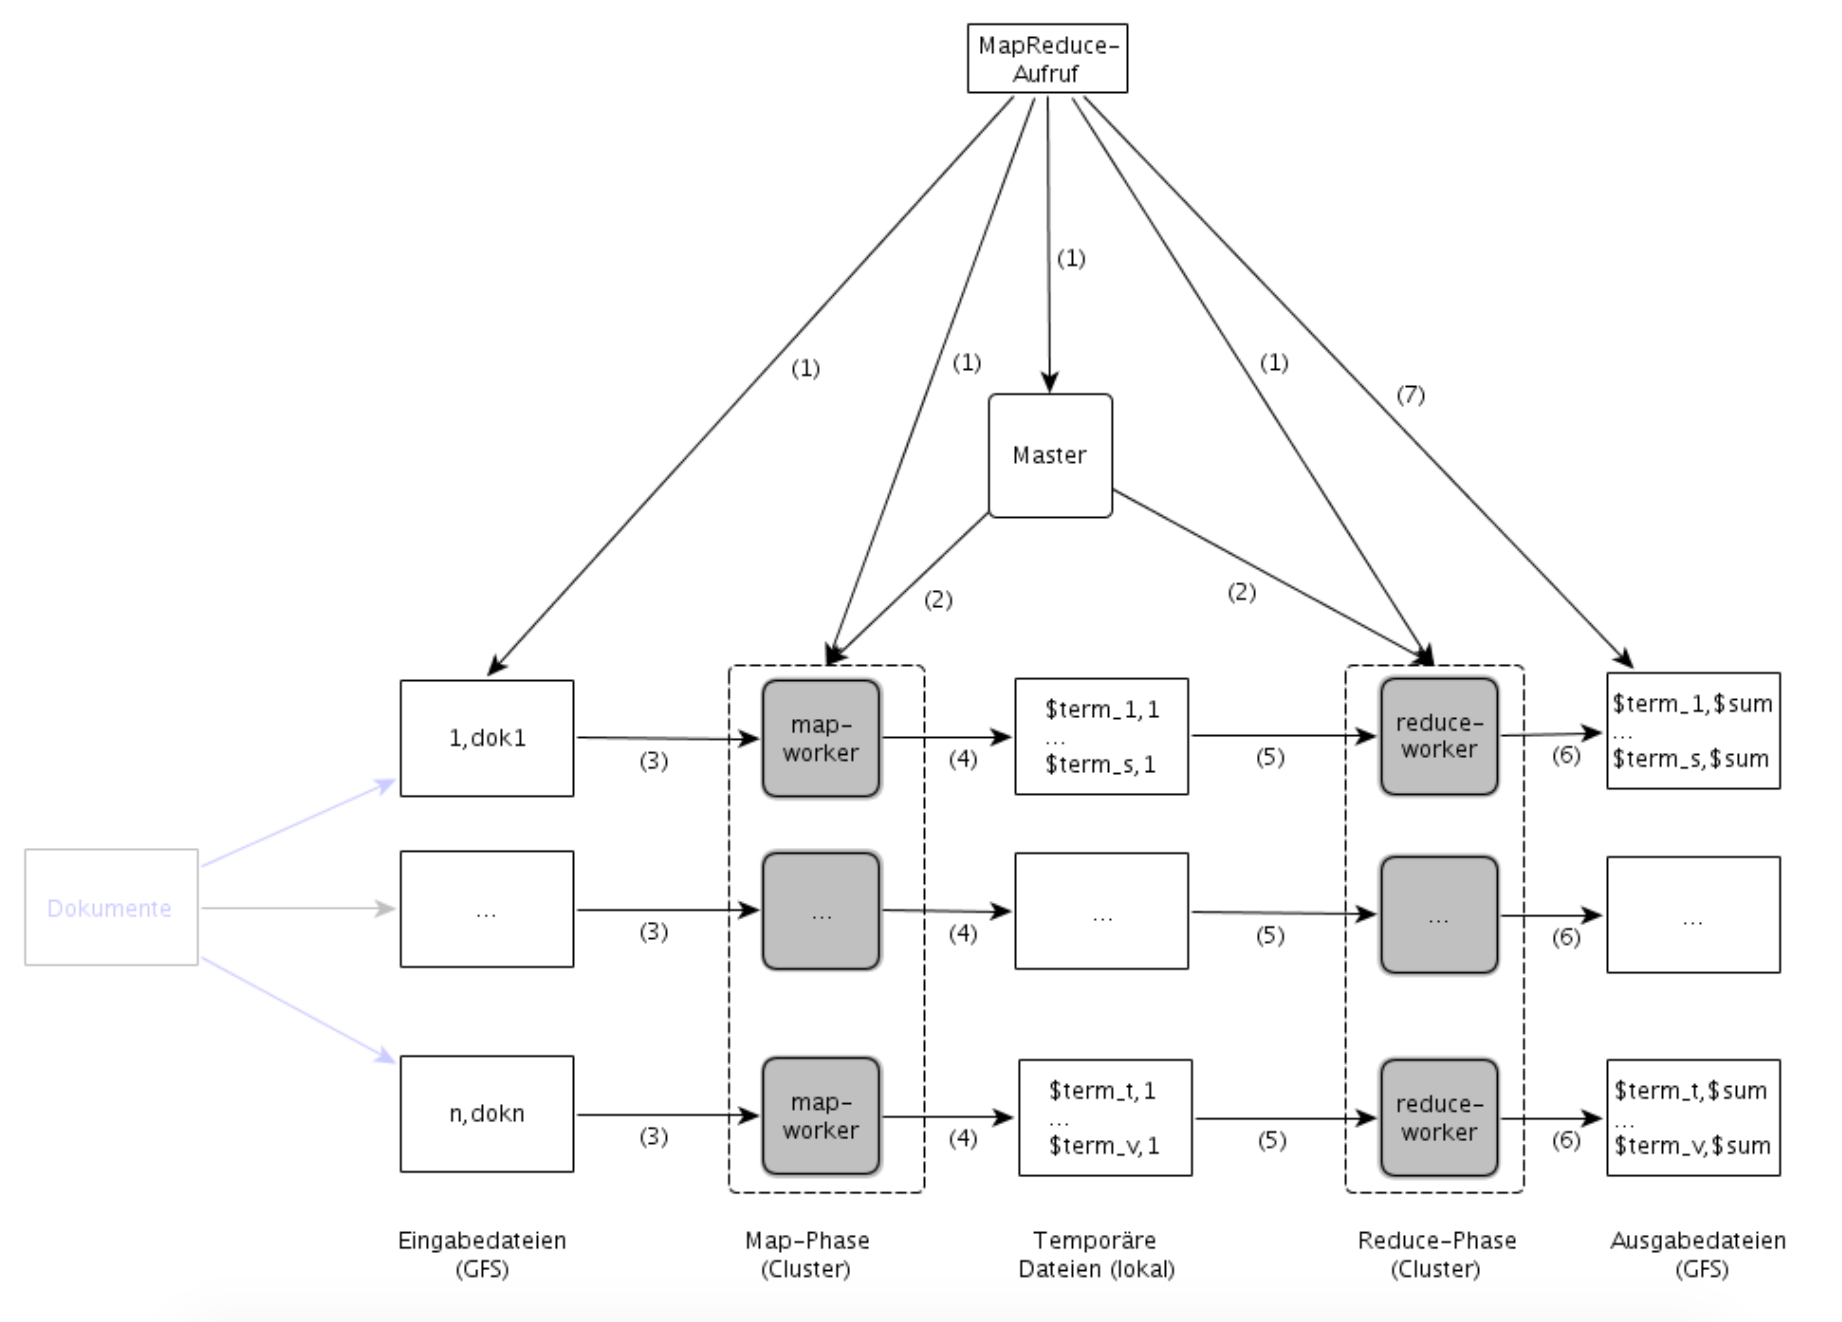
\includegraphics[width=0.9\textwidth]{picture/map_reduce_system_example.png}
	\caption{Systemübersicht eines Map-Reduce System \cite{Bethge2009}}
	\label{graphicMapReduceSystem}
\end{figure}

Weiterhin ist auf Abbildung~\ref{graphicMapReduceSystem} in Schritt zu erkennen, dass jeder Worker, der eine Map-Aufgabe ausführt, eine Teilmenge der zu verarbeitenden Gesamtdatenmenge als Eingabe erhält. Die Daten müssen dazu in Form von Schlüssel-Wert Paaren gespeichert sein. Diese werden dann gemäß der vom Nutzer spezifizierten UDF verarbeitet. Als Ausgabe werden keine, ein oder mehrere Schlüssel-Wert Paare durch die map-Funktion produziert und im lokalen Speicher der jeweiligen Worker gespeichert. Aufgrund der Aufteilung der Gesamtdatenmenge in kleinere, von einander unabhängig prozessierbare Mengen, kann die Map-Phase parallelisiert ablaufen. Dabei werden auf jedem Worker des Clusters verschiedene Teilmengen der Eingabedaten verarbeitet. 

Nach Beendigung der Map-Phase folgt die Shuffle-Phase, auch auch Repartitionsphase genannt. Diese ist in Abbildung~\ref{graphicMapReduceSystem} als Schritt 4 gekennzeichnet. Während dieser werden die durch die Map-Funktion produzierten Schlüssel-Wert Paare gemäß ihrer Schlüssel gruppiert. Wenn der Speicherbedarf für alle Schlüssel-Wert Paare einer Gruppe größer ist als der verfügbare Speicher auf einem Worker werden mehrere Gruppen mit demselben Schlüsselwert gebildet. Jede Gruppe wird anschließend in Schritt 5 auf verfügbare Worker übertragen, um die anschließende Anwendung der reduce-Funktion zu ermöglichen.

Die reduce-Funktion, die durch Schritt 6 dargestellt wird, wird auf jede in der Shuffle-Phase erzeugten Gruppe von Schlüssel-Wert Paaren angewendet. Die spezifizierte UDF wird auf die Werte aller Schlüssel-Wert Paare einer Gruppe angewendet. Als Ausgabe wird entweder keine, ein oder mehrere Schlüssel-Wert Paare produziert. 

Die Gesamtausgabe des Map-Reduce Programms besteht aus allen durch reduce-Funktionen produzierten Schlüssel-Wert Paaren.

Aufgrund der sehr genau festgelegten Programmstruktur, die zur Nutzung von Map-Reduce eingehalten werden muss wird der Anwender gezwungen einen Datenverarbeitungsprozess auf mehrere aufeinanderfolgende Map-Reduce Instanzen zu verteilen, wenn dieser zu komplex ist. 
 
Seit seiner Einführung im Jahr 2004 wurde das Map-Reduce Paradigma erweitert und bietet nun mehr Flexibilität, da es um weitere Funktionen zweiter Ordnung ergänzt wurde, die zusätzliche Datentransformationen ermöglichen. Aufgrund des Einsatzes von Map-Reduce in Hadoop \cite{HadoopWebsite} und anderen Systemen wie beispielsweise Spark \cite{Zaharia2010} bleibt es aber eines der dominanten Paradigmen bei der Verarbeitung großer Datenmengen. Auch Apache Flink \cite{FlinkWebsite} nutzt eine ähnliche Funktionsweise, um die parallelisierten Datenströme zu verwalten.

%Andere Systeme (Hadoop, Astercks, Spark etc)
Neben den bereits erwähnten Systemen Apache Hadoop und Apache Flink existieren weitere populäre Systeme, beispielsweise Apache Spark \cite{SparkWebsite, Zaharia2010}, Apache Storm \cite{StormWebsite, Jones2013} oder Asterix \cite{AsterixWebsite, Alsubaiee2012}. Diese unterscheiden sich bereits in ihrer Architektur. Während Apache Hadoop das Map-Reduce Paradigma sehr fixiert umsetzt und somit dem Nutzer nur eingeschränkte Mittel zur Spezifizierung seines Programmes lässt, setzen Systeme wie Apache Spark und Apache Flink das Map-Reduce Paradigma flexibler ein. Nachfolgend wird ein kurzer Überblick über die Funktionsweise der genannten Systeme gegeben. 

\textbf{Apache Hadoop}. Apache Hadoop implementiert das Map-Reduce System im Rahmen eines freien Projekts. Dabei können sowohl die Map- als auch die Shuffle- und Reducephase vom Nutzer individuell konfiguriert werden. Als freier Ersatz für GFS nutzt Hadoop das Dateisystem Hadoop Distributed File System (HDFS). In der Basisversion ermöglicht Hadoop lediglich Stapelverarbeitungen, echtzeitnahe Datenverarbeitung ist nicht vorgesehen. Hadoop wird in diversen Firmen genutzt, zum Beispiel verwendet Facebook das System zur Analyse von Datenmengen von bis zu 100 Petabyte \cite{Borthakur2013}.

\textbf{Apache Spark}. Apache Spark ist eine allgemeine Datenverarbeitungsplattform. Es beinhaltet mehr Funktionen zweiter Ordnung als Hadoop, es gibt also mehr Möglichkeiten verschiedene Datentransformationen auszuführen. Im Gegensatz zu Hadoop ermöglicht es neben der Stapelverarbeitung weitere Anwendungen wie zum Beispiel maschinelles Lernen. Des weiteren ist ebenfalls möglich Spark mit anderen Bibliotheken zu ergänzen. Diese Eigenschaften machen Spark gegenüber Hadoop für viele Anwendungszecke überlegen. 

\textbf{Apache Storm}. Apache Storm ist ein Datenverarbeitungssystem, das speziell auf die schnelle echtzeitnahe Verarbeitung von Daten ausgelegt ist. Ein Storm-Programm hat die Form eines direkten, azyklischen Graphs, dessen Kanten Datenströme darstellen. Ein Storm-Programm kann als datentransformierende Pipeline bezeichnet werden. Ein Storm-Programm entspricht einer Implementierung eines abstrakten Map-Reduce-Jobs. Im Unterschied zu einem Map-Reduce Job läuft ein Storm-Programm, bis es beendet wird. Dies unterstreicht den Einsatzzweck für echtzeitnahe Verarbeitung von Daten, die ohne Zeitbegrenzung generiert werden.

\textbf{Asterix}. 

%Hadoop, z.b. bei 
\subsection{Apache Flink}
\label{sec:ApacheFlink}
%Flink einführen + allgemein beschreiben
Ein Datenverarbeitungssystem, das auf eine massiv parallelisierte Verarbeitung von großen Datenmengen spezialisiert ist, ist Apache Flink. Es ging 2014 aus Stratosphere hervor \cite{BraunWebsite}, einem Forschungsprojekt, das seit 2010 kooperativ von Forschern verschiedener Universitäten entwickelt wurde \cite{Battre2010, Alexandrov2014}. Seit Januar 2015 ist Apache Flink ein Top-Level Projekt der Apache Software Foundation \cite{ApacheFlinkBlogEntry}. 
Ähnlich wie andere Systeme ermöglicht es Apache Flink bereits vorhandene Daten in einem \textit{Batch}-Verfahren zu analysieren. Darüber hinaus können jedoch auch in Echtzeit zu verarbeitende Daten im Rahmen eines \textit{Streaming}-Verfahrens prozessiert werden. 

Die Hauptkomponenten von Apache Flink sind die Flink-Laufzeitumgebung (engl. \textit{Flink Runtime} ) und der Flink-Optimierer (engl. \textit{Flink Optimizer}). Darüber hinaus verfügt Flink über Programmierschnittstellen für die Hochsprachen Java, Python und Scala, mithilfe derer Nutzer Flink-Programme spezifizieren können. 

%Konzept: 2nd order functions, UDFs, Operatoren
Flink implementiert das vom Map-Reduce System bekannte Schema von Funktionen zweiter Ordnung und gekapselten nutzerdefinierten Funktionen erster Ordnung. Dabei beschreibt die Funktion zweiter Ordnung die Art der Datentransformation, die UDF definiert die vom Nutzer spezifizierte Verarbeitungslogik, die auf die Daten angewendet werden soll. Im Gegensatz zum Map-Reduce System verfügt Flink jedoch nicht nur über die Funktionen zweiter Ordnung Map und Reduce, sondern bietet insgesamt 15 verschiedene Datentransformationen. Diese werden als Operatoren bezeichnet. Weitere wichtige Operatoren neben Map und Reduce sind beispielsweise Cross, Match und CoGroup, die in Abbildung~\ref{graphicFlinkOperators} dargestellt sind. Jeder Operator besteht also aus jeweils einer spezifischen Transformation sowie einer eingebetteten UDF. Zusätzlich besitzen Operatoren eine Eingabe- sowie eine Ausgabedatenmenge in Form eines Datenstroms. Ein Flink-Programm wird als ein Datenfluss in Form eines direkten und azyklischen Graphen dargestellt, dessen Knoten Operatoren und dessen Kanten Datenströme darstellen. \textcolor{blue}{Ref auf Abbildung eines Beispieldatenstroms.}. Dieser wird \textit{Operator DAG} genannt. 

\begin{figure}[h]
	\centering	
	\captionsetup{justification=centering,margin=2cm}
	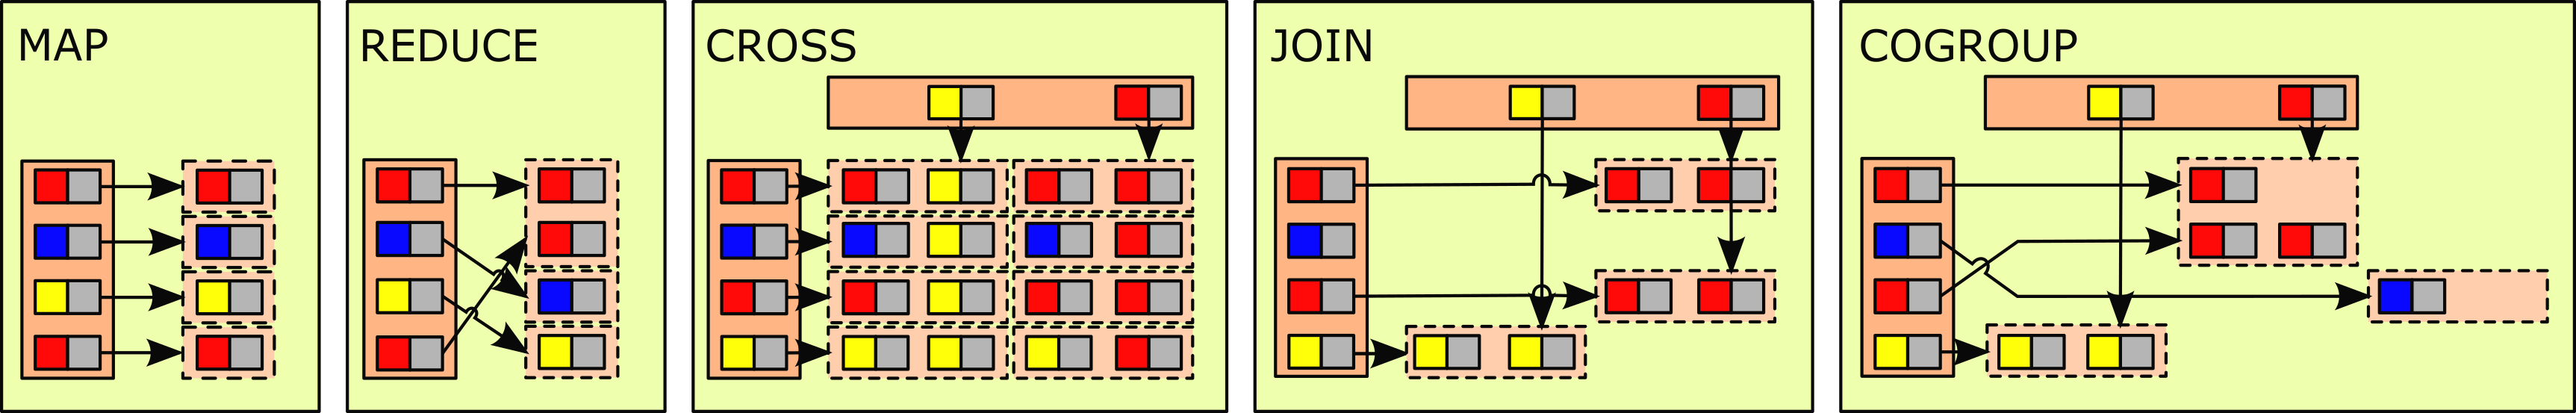
\includegraphics[width=0.9\textwidth]{picture/flink_operators.png}
	\caption{Funktionen zweiter Ordnung: (a) Map, (b) Reduce, (c) Cross, (d) Match, and (e) CoGroup \cite{Hueske2012}}
	\label{graphicFlinkOperators}
\end{figure}

%Optimizer
Der Flink-Optimierer erhält den mithilfe einer Programmierschnittstelle spezifizierten Operator DAG als Eingabe. Die Aufgabe des Flink-Optimierers ist die Umwandlung des Operator DAG in einen parallelisiert ausführbaren Datenfluss, den \textit{OptimizedPlan}. Der OptimizedPlan soll möglichst stark parallelisierbar sein, damit eine effiziente Verarbeitung des OptimizedPlans durch die Flink-Laufzeitumgebung ermöglicht werden kann. Um einen OptimizedPlan zu erhalten werden abhängig von den verwendeten Operatoren programmspezifische Optimierungen vorgenommen. Dabei wird für jeden Operator auf Basis seiner Eingabedaten festgelegt, mit welcher internen Implementierung der Operator ausgeführt wird. Ein Beispiel dafür wäre die Ausführung eines Join-Operators wahlweise als Sort-Merge-Join oder als Hash-Join. Weitere Optimierungen umfassen die Wahl des Datenaustauschs zwischen den Operatoren sowie die Auswahl der Programmpunkte, an denen Zwischenergebnisse gespeichert werden. Außerdem wird versucht Daten, die durch einen Operator sortiert oder partioniert wurden, mit derselben Sortierung weiterzuverwenden, um weitere Sortier- oder Partionierungsprozesse zu vermeiden. Ist der optimale OptimizedPlan ermittelt wird er zu einem \textit{JobGraph}, einem direkten azyklischen Graphen bestehend aus Operatoren und Zwischenergebnissen als Knoten, umgewandelt. Ein Bespiel für einen JobGraph wird in Abbildung~\ref{graphicJobExecution} gezeigt. Dieser wird dann von der Flink-Runtime verarbeitet.

\begin{figure}[h]
	\centering
	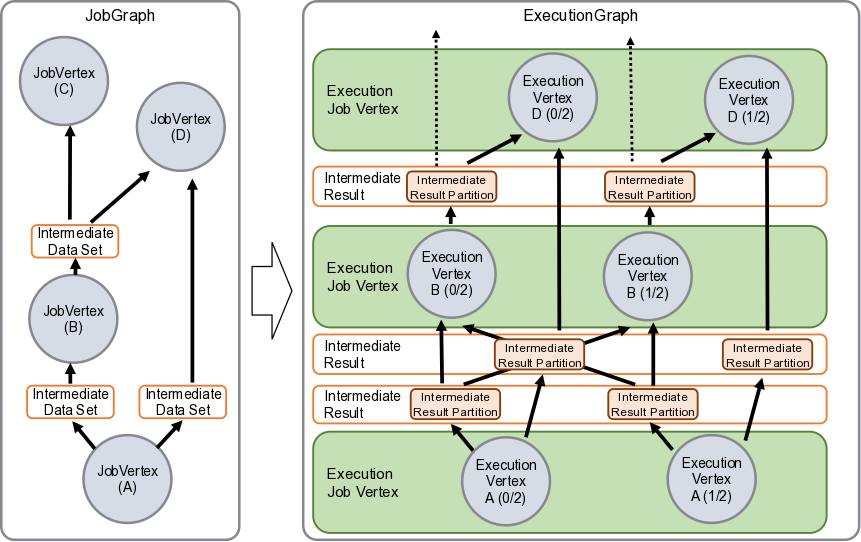
\includegraphics[width=0.9\textwidth]{picture/flink_job_and_execution_graph.png}
	\caption{Modell eines Jobgraphs und des dazugehörigen ExecutionGraphs}
	\label{graphicJobExecution}
\end{figure}

%Konzept: JobManager: Masternode <-> Workernodes. Wie funktioniert die Parallelität?
Flink nutzt ebenso wie das Map-Reduce System eine Master-Worker Architektur zur Organisation des Netzwerkes, auf dem das Flink-Programm ausgeführt wird. Abbildung~\ref{flinkArchitecture} zeigt eine Übersicht der Systemstruktur von Flink. Der Master-Knoten, auch \textit{Jobmanager} genannt, verwaltet dabei eine variable Anzahl an Worker-Knoten, \textit{TaskManager} genannt. Gemäß der Master-Worker Architektur weist der JobManager den einzelnen TaskManagern Programmteile zu, die diese dann ausführen. Der Status der Ausführung wird vom JobManager überwacht. Fällt ein TaskManager aus werden dessen Aufgaben von anderen Worker-Knoten übernommen bzw. wiederholt. Eine Besonderheit des Flink-Systems ist der Datenaustausch zwischen Workern in Form von Datenströmen untereinander. 

Wird ein Flink-Programm ausgeführt, wird nachdem die Optimierung beendet ist das System gemäß nutzerdefinierter Prämissen wie dem Grad der Parallelität initialisiert. Der JobManager erhält den vom Flink-Optimizer generierten JobGraph als Eingabe. 
Dieser wird, wie in Abbildung~\ref{graphicJobExecution} dargestellt, in einen parallel strukturierten \textit{ExecutionGraph} transformiert. Für jeden Knoten des Jobgraphs wird ein \textit{ExecutionJobVertex} erstellt. Dieser verantwortet die Ausführung des durch den Knoten repräsentierten Operators sowie die Weitergabe der, aus der Anwendung des Operators auf die Eingabedaten resultierenden, Zwischenergebnisse. Dabei werden \textit{n ExecutionVertices} genutzt, wobei \textit{n} dem vom Nutzer festgelegten Grad der Parallelität entspricht. Jeder ExecutionVertex übernimmt die Ausführung einer der parallelisierten Verarbeitungsinstanzen des Operators. Dazu wird ein vom JobManager bestimmter Worker-Knoten genutzt. Der ExecutionJobVertex garantiert die komplette Ausführung des Operators auf der gesamten Eingabedatenmenge, indem der Status jedes ExecutionVertex verfolgt wird. Sollte einer der ExecutionVertices ausfallen wird die gerade verarbeitete Ausführungsinstanz an andere ExecutionVertices delegiert. Darüber hinaus beinhaltet der ExecutionGraph die Zwischenergebnisse, die zwischen der Anwendung verschiedener Operatoren erstellt werden. Dadurch ist jederzeit bekannt, ob die Bedingungen für die Ausführung eines weiteren Operators gegeben ist, oder ob noch nicht alle Eingabedaten in Form von Zwischenergebnissen verfügbar sind.

\begin{figure}[h]
	\centering
	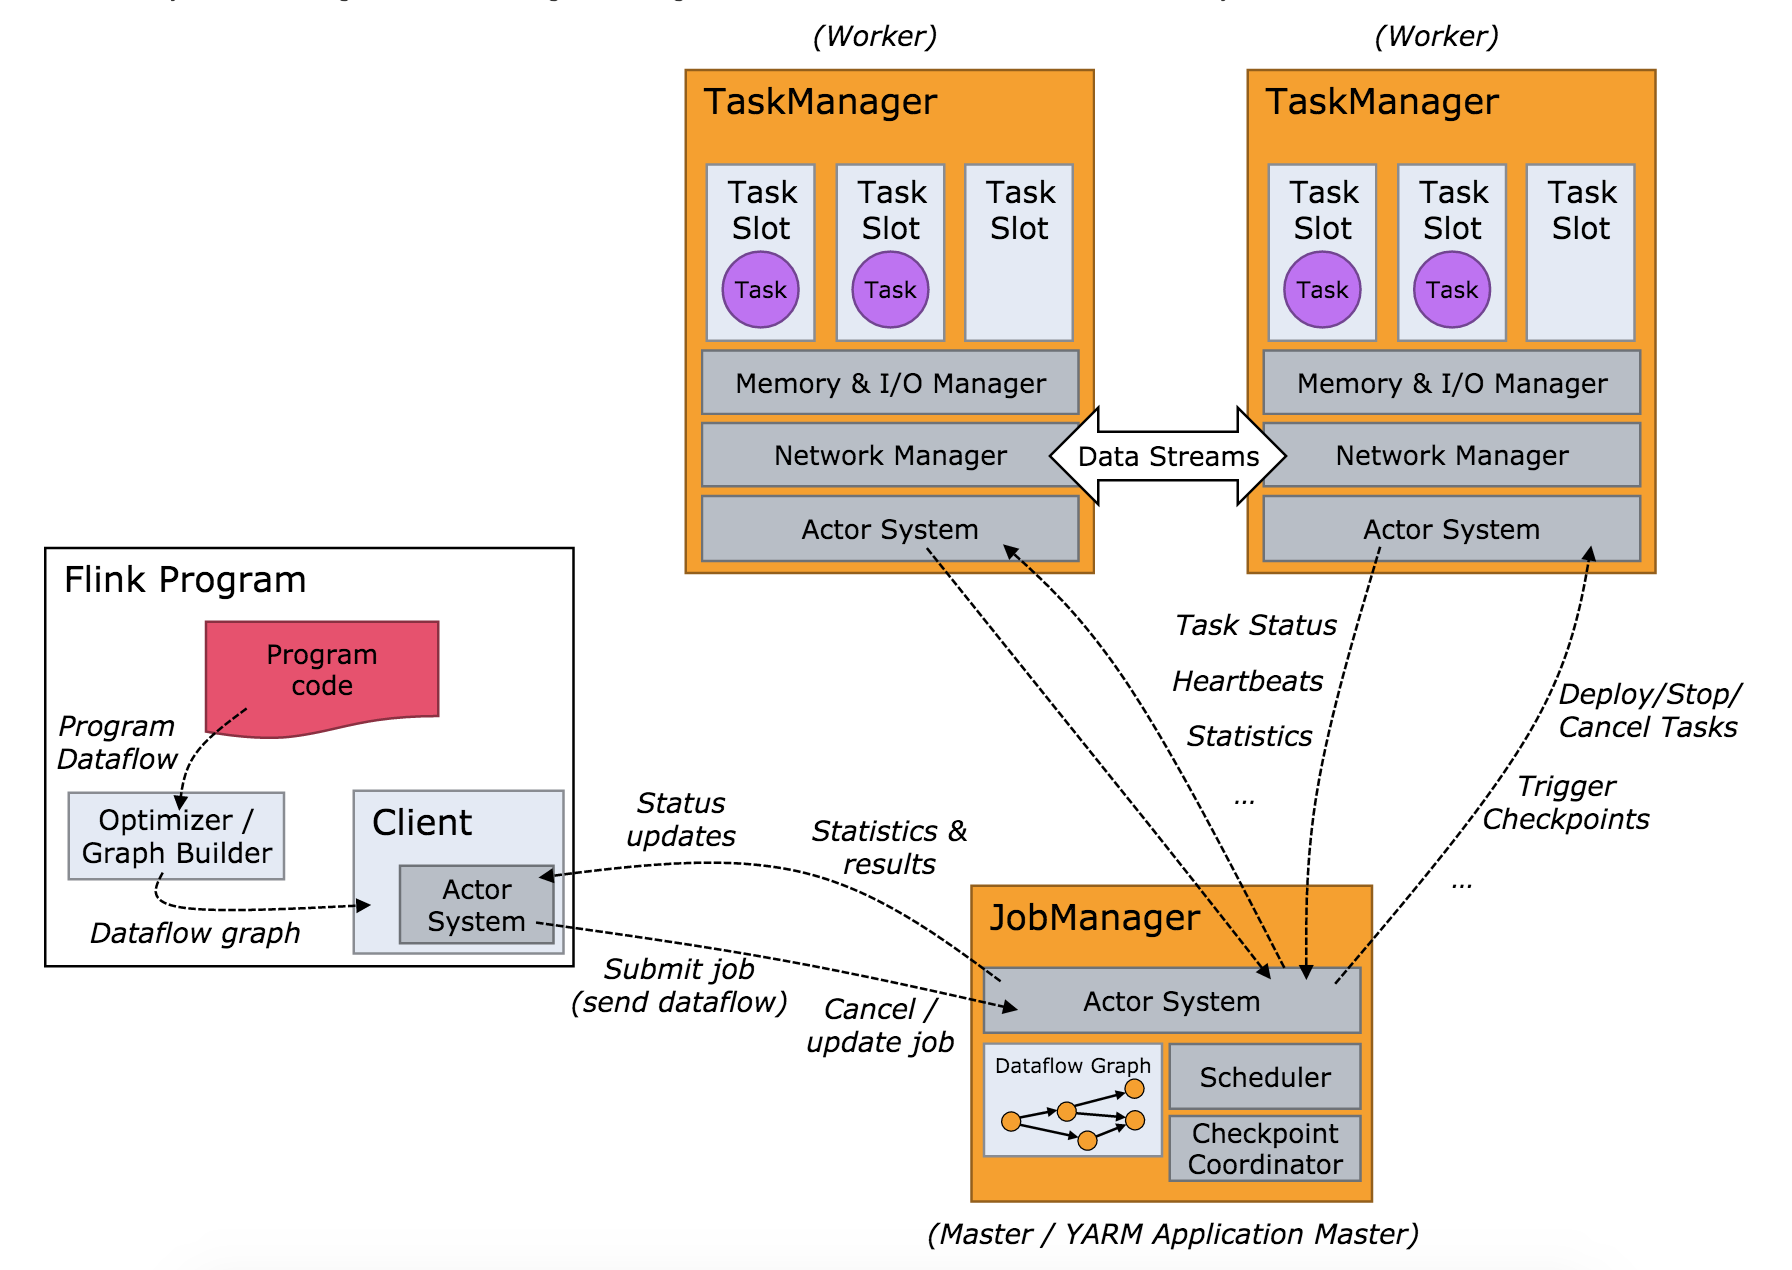
\includegraphics[width=0.9\textwidth]{picture/flink_architecture.png}
	\caption{Systemübersicht bei der Ausführung eines Flink-Programms \cite{FlinkArchitecureImage}}
	\label{flinkArchitecture}
\end{figure}

\subsection{Python}
\label{sec:Python}
Python ist eine höhere, interpretierte Programmiersprache, die seit 1989 existiert, quelloffen ist und fortwährend weiter entwickelt wird. Obwohl Python eine imperative Sprache ist, können auch objektorientierte und funktionale Programmierparadigmen verwendet werden. Jedes Python-Programm wird bei der Ausführung mittels des Python-Interpreters in Bytecode umgewandelt. Dieser ist plattformunabhängig lauffähig, so dass Python-Programme ohne weitere Modifizierung auf mehreren Systemen lauffähig sind. Eine weitere Eigenschaft von Python sind die sehr umfangreiche Standardbibliothek sowie die Erweiterbarkeit um Module und Bibliotheken. Des weiteren gibt es mit der Python-API die Möglichkeit Python-Code durch C- beziehungsweise C++-Bibliotheken zu erweitern \cite{Martelli2006}. Unter anderem aufgrund der maschinennahen Umsetzung und der effizient implementierten Compiler von C beziehungsweise C++ besitzen diese Sprachen einen Leistungsvorteil gegenüber anderen höheren Programmiersprachen. Dies kann in Python genutzt werden, indem leistungsintensive Programmteile direkt als C- oder C++-Code eingebunden und ausgeführt werden. Ein weiterer Vorteil von Python ist die starke Typisierung und daraus resultierend die bessere Optimierung des Codes bei der Übersetzung durch den Python-Interpreter. Zusätzlich nutzt Python Duck-Typing, also die Typbeschreibung eines Objekts alleinig durch das Vorhandensein bestimmter Methoden beziehungsweise Attribute, was die Nutzbarkeit der Typisierung durch den Entwickler vereinfacht.

Ein Schwachpunkt von Python im Bezug auf die schnelle Verarbeitung großer Datenmengen ist die nicht auf automatisierte Parallelisierung ausgelegte Architektur. Daraus resultiert eine unzureichende Skalierbarkeit der Datenverarbeitung, sobald Daten, deren Größe die Arbeitsspeichergröße der ausführenden Maschine übersteigt, verarbeitet werden müssen. Dies ist insbesondere im Zuge der in Abschnitt~\ref{sec:GrosseDatenmengen} aufgezeigten Entwicklung hin zu größeren zu verarbeitenden Datenmengen relevant. Entwicklungen, die eine bessere Parallelisierung und damit einhergehend eine bessere Skalierbarkeit von Python Projekten zum Ziel haben, sind jedoch meist nicht universal anwendbar oder bieten nicht den Funktionsumfang von Big-Data Systemen \cite{ParallelPythonWebsite, DispyWebsite}. Die Funktionalität dieser Entwicklungen wird dabei durch Module bereitgestellt, da sie nicht als Grundfunktion in Python existiert sondern projektweise hinzugefügt werden muss. Dies erhöht den zu leistenden Anpassungs- und Entwicklungsaufwand im Vergleich zu anderen Systemen, die mit Rücksicht auf diese Anwendungsfälle konzipiert wurden.

Trotzdem nutzen viele Nutzer, die Big-Data Anwendungen entwickeln, Python \cite{Millman2011}. Einerseits ist die Sprache ein seit vielen Jahren bewährtes Werkzeug, das durch Nutzung von Bibliotheken wie SciPy und NumPy effizient implementierbare Algorithmen ermöglicht, ohne dass alle genutzten Funktionen selbst programmiert werden müssen. Andererseits verhindern die erwähnten Einschränkungen bezüglich der Parallelisierbarkeit einen unbeschränkten Einsatz zur Lösung von datenintensiven Problemen und Prozessen. Weitere Gründe für das Festhalten von Python sind zum Beispiel die Möglichkeit zur Einbindung von Fortran und die bei Nutzung neuerer Systeme notwendige Reimplementation bereits existierender Lösungen. Die Kosten-Nutzen-Relation bei einer Nutzung anderer Systeme wie zum Beispiel Apache Flink muss dabei projektabhängig und individuell aufgestellt werden. Diese Relation wird im Rahmen dieser Bachelorarbeit für die Implementation einer Satellitenbildanalyse mittels des in Kapitel~\ref{cha:AlgorithmForSatellitePictureAnalysis} beschriebenen Algorithmus evaluiert.

%----------------------------------------------------------------------------------

\chapter[Algorithmus zur Analyse von Pixelzeitreihen]{Beschreibung und Umsetzung des Algorithmus zur Analyse von Pixelzeitreihen}
\label{cha:AlgorithmForSatellitePictureAnalysis}
\section[Beschreibung des Algorithmus]{Beschreibung des Algorithmus zur Analyse von Pixelzeitreihen}
%Einleitung: Kurze, grobe Beschreibung des Algorithmus, kurze Wiederholung relevante Geographische Grundlagen.
Das Ziel des in dieser Bachelorarbeit implementierten und evaluierten Algorithmus ist die Analyse einer Veränderung der Flora einer geographischen Region. Auf Basis dieser Analyse sollen dann zukünftige Werte prognostiziert werden. Als Grundlage der Analyse dienen Satellitenbilder der jeweiligen Region. Diese Satellitenbilder werden bezüglich Veränderungen des Vegetationsindexes der jeweiligen Region untersucht. Die zu diesem Zweck genutzte Analyse ist eine kombinierte Anwendung von \textit{Support Vector Regression} (SVR) \cite{Basak2007} und dem \textit{Continuous Monitoring of Forest Disturbance Algorithm} (CMFDA) \cite{Zhu2012}. 

%Ziel der Analyse

%Beschreibung SVR

%Beschreibung Zhu
Der \textit{Continuous Monitoring of Forest Disturbance Algorithm} wurde 2012 von Zhu et al. vorgestellt \cite{Zhu2012}. Er wurde entwickelt, um die Veränderung von Waldbeständen geographischer Regionen kontinuierlich zu überwachen und atypische Veränderungen zu entdecken. Aus den Szenen, die analysiert werden sollen, werden die Bilder der einzelnen Spektralbänder extrahiert. Jedes dieser Bilder wird in einzelne Pixel geschnitten. Diese Pixel werden gemäß des jeweiligen Spektralbands und der Pixelkoordinate gruppiert, so dass Pixelzeitreihen entstehen. Anschließend muss jede Pixelzeitreihe gemäß dem Entstehungszeitpunkt gruppiert werden. Eine Analyse mittels CMFDA umfasst acht Schritte, die im folgenden kurz beschrieben werden.

\textbf{1. Vorverarbeitung von Daten.} Für die Durchführung der Analyse müssen die genutzten Satellitenbilder geometrisch normalisiert und atmosphärisch korrigiert sein. Für Szenen des Landsat-Systems wird die geometrische Korrektheit angenommen und die atmosphärische Korrektheit durch die Anwendung des Landsat Ecosystem Disturbance Adaptive Processing System erreicht.

\textbf{2. Wolken-, Wolkenschatten- und Schneekorrekturen.} Da Wolken, Wolkenschatten und Schnee Störfaktoren darstellen, die die Ergebnisse der Analyse verfälschen können, müssen diese vorher automatisiert ermittelt und die betreffenden Pixel von der Analyse ausgeschlossen werden. Dies wird mithilfe eines zweistufigen Algorithmus erreicht, der in einem ersten Schritt bereits potenzielle Wolken- bzw. Wolkenschattenpixel erkennt \cite{Zhu2012a}. Im zweiten Schritt werden diese dann eindeutig identifiziert, indem Informationen über die Temperatur der jeweiligen Pixel mit einbezogen werden. Des weiteren werden Toleranzgrenzen um die nicht validen Pixel herum gebildet, die bei der Analyse ebenfalls nicht berücksichtigt werden. Dadurch wird die Fehlerquote bei der Kategorisierung valider Pixel reduziert.

\textbf{3. Prognose des Oberflächenreflektionsmodell.} Nach der Bereinigung der Szenen von Wolken, Wolkenschatten und Schnee wird für alle validen Pixel aller Szenen ein Oberflächenreflektionsmodell aufgestellt. Voraussetzung ist, dass ausreichend viele Szenen vorhanden sind, auf denen der Pixel als valide klassifiziert wurde. Dann wird mithilfe eines harmonischen Modells die Oberflächenreflektion zum Zeitpunkt der Aufnahme ermittelt, so dass der Pixel entsprechend korrigiert werden kann. 

\textbf{4. Definition einer stabilen Waldschablone.} Um zu prüfen, ob ein Pixel einer Szene Wald abbildet oder nicht muss ein Vergleichswert zur Feststellung dieses Wertes definiert werden. Dies geschieht, indem spezifische Charakteristika von auf Satellitenbildern abgebildeten Wäldern definiert werden. \textcolor{blue}{Mehr schreiben}.

\textbf{5. Vorhersage von zukünftigen Landsat-Szenen.} Angenommen, die Landoberfläche hat sich bis zum Zeitpunkt der nächsten verwertbaren Landsat-Aufnahme nicht geändert, so ist es möglich die Oberflächenreflektion jedes Pixels für jedes Spektralband zu prognostizieren.

\textbf{6. Algorithmische Erkennung von Veränderungen.}



%Beschreibung Kombination der beiden Methoden

%Die Satellitenbilder, die die Ausgangsdaten der Analyse des Vegetationsindexes einer Region darstellen, werden durch Landsat-Fernerkundungssatelliten aufgenommen. Diese kreisen so um die Erde, dass alle 16 Tage dieselbe geographische Region. Um eine Entwicklung mehrerer Jahre zu aufzuzeigen benötigt der Analysealgorithmus demzufolge mehrere Dutzend Satellitenaufnahmen der betreffenden Region. Diese müssen darüberhinaus für die Analyse aufbereitet werden. Diese Aufbereitung umfasst zum einen das Beschneiden der Szenen, so dass lediglich der Zielbereich verbleibt, zum anderen die Korrektur bzw. Filterung des Bildinhaltes. Denn aufgrund von Störfaktoren wie sphärischen Reflektionen oder Wolkenbildung sind möglicherweisenicht alle in den Szenen enthaltenen Pixel durch die Analyse verwertbar. Die fehlenden Werte werden im Zuge der Analyse approximiert, so dass vollständige Pixelzeitreihen zur Vorhersage zukünftiger Werte genutzt werden können. 

\section{Umsetzung des Algorithmus mit Apache Flink}
\subsection{Nutzung der Java-Programmierschnittstelle}
\subsection{Nutzung der Python-Programmierschnittstelle}
\section{Umsetzung des Algorithmus in Python}
%Einordnung als Big-Data Problem (Einordnung am GfZ bei GeoMultiSens)
Die Analyse von Satellitenbildern erfordert die Verarbeitung großer Mengen komplexer Rohdaten, \textcolor{green}{die nahezu in Echtzeit verfügbar sind}. Aufgrund dieser Charakteristika handelt es sich bei dieser Analyse um ein \textcolor{blue}{Big-Data Problem}. Denn alle vier Kriterien, die ein solches charakterisieren sind erfüllt.
\newline
Bei der Analyse von Satellitenbildern sind die Merkmale Datengröße und Datenkomplexität sowie die schnelle Verarbeitung der Daten von Bedeutung. Abhängig von der Anzahl der genutzten Bilder sind die zu verarbeitenden Datenmengen sehr groß. Ein Bild besitzt im Regelfall abhängig vom Satellitenmodell, das die Aufnahme gemacht hat, eine Größe von 750 Megabyte bis zu 1,5 Gigabyte. Um eine Entwicklung zu untersuchen werden jedoch viele dieser Bilder in die Untersuchung mit einbezogen, so dass die zu verarbeitende Datenmenge kontinuierlich ansteigt. Dieser kontinuierliche Anstieg entsteht dadurch, dass aktuell mehrere Satelliten mit der Fernerkundung der Erde fortfahren und so in kurzen Intervallen neue Bilder zur Verfügung stehen, die im Rahmen der Analyse verwendet werden sollen. \textcolor{green}{Quelle}.
%Big Data + Eigenschaften,



%Datenstrom mit Flink Operatoren
\begin{tikzpicture}[>=latex']
        \tikzset{block/.style= {draw, rectangle, align=center,minimum width=2cm,minimum height=1cm},
        rblock/.style={draw, shape=rectangle,rounded corners=1.5em,align=center,minimum width=2cm,minimum height=1cm},
        input/.style={ % requires library shapes.geometric
        draw,
        trapezium,
        trapezium left angle=60,
        trapezium right angle=120,
        minimum width=1cm,
        align=center,
        minimum height=1cm
    },
        }
        \node [rblock]  (start) {Input data};
        %Filter the data
        \node [block, below =1cm of start, label={[name=l] Filter the data}, draw] (filterDataInner) {filter('valid')};
        \node [fit=(filterDataInner) (l), draw] (filterDataOuter) {};
        %Group the data
        \node [block, below =1cm of filterDataOuter, label={[name=l] Group the filtered data}, draw] (groupDataInner) {groupBy('geographic position(maybe as a tile)')};
        \node [fit=(groupDataInner) (l), draw] (groupDataOuter) {};
        %Sort every grouped dataSet
        \node [block, below =1cm of groupDataOuter, label={[name=l] Sort every grouped dataSet}, draw] (sortDataInner) {sortPartition('time')};
        \node [fit=(sortDataInner) (l), draw] (sortDataOuter) {};
        %Approx the missing data
        \node [block, below = 1cm of sortDataOuter, label={[name=l] Approx. the missing data}, draw] (approximateDataInner) {groupReduce()};
        \node [fit=(approximateDataInner) (l), draw] (approximateDataOuter) {};
        %Predict the future data
        \node [block, below = 1cm of approximateDataOuter, label={[name=l] Predict the future data}, draw] (predictDataInner) {groupReduce()};
        \node [fit=(predictDataInner) (l), draw] (predictDataOuter) {};
        %Sink the data
        \node [rblock, below = 1cm of predictDataOuter, draw] (end) {Sink};

        \node [coordinate, below right =1cm and 1cm of start] (right) {};  %% Coordinate on right and middle
        \node [coordinate,above left =1cm and 1cm of start] (left) {};

%% paths
        \path[draw,->] (start) edge (filterDataOuter)
                    (filterDataOuter) edge (groupDataOuter)
                    (groupDataOuter) edge (sortDataOuter)
                    (sortDataOuter) edge (approximateDataOuter)
                    (approximateDataOuter) edge (predictDataOuter)
                    (predictDataOuter) edge (end)
                    ;
\end{tikzpicture}

%Minimal diagram example
%\begin{tikzpicture}[nodes=draw]
%    \node [label=label1,draw] (node1) {Node1};
%\end{tikzpicture}

%----------------------------------------------------------------------------------

\chapter{Evaluierung}
%Korrektheit, Performant, welche Impl. anderen überlegen [bei welchen Gesichtspunkten]
\section{Versuchsbeschreibung}
Beschreibung + Begründung für meine Versuchsbedingungen
\section{Auswertung}
Beschreibung und Bewertung der Ergebnisse meiner Untersuchungen

\chapter{Fazit}
Fazit und Ausblick
z.b. Vergleich mit anderen Untersuchungen

